\documentclass[final,3p,10pt,nopreprintline]{elsarticle}
\usepackage[T1]{fontenc}
\usepackage{lmodern}
\usepackage{amsmath,amssymb,booktabs,array,graphicx,xurl}
\usepackage{float}
\usepackage[hidelinks]{hyperref}
\usepackage[section]{placeins}
\journal{Array}
\newcolumntype{L}[1]{>{\raggedright\arraybackslash}p{#1}}
\setlength{\emergencystretch}{2em}
\setlength{\belowcaptionskip}{5pt}
\raggedbottom


\makeatletter
\expandafter\def\csname r@sup:protocol\endcsname{{S1}{1}{}{}{}}
\expandafter\def\csname r@sup:comparators\endcsname{{S2}{1}{}{}{}}
\expandafter\def\csname r@sup:serving\endcsname{{S3}{2}{}{}{}}
\expandafter\def\csname r@sup:explanation\endcsname{{S4}{2}{}{}{}}
\expandafter\def\csname r@sup:diagnostics\endcsname{{S5}{3}{}{}{}}
\makeatother




\begin{document}

\nocite{r1,r2,r3,r4,r5,r20,r27,r28,r29,r6,r7,r8,r9,r10,r11,r12,r21,r22,r23,r24,r25,r13,r14,r15,r17,r18,r19,r16,r26,r30}

\begin{frontmatter}\title{Multiscale endpoint context and prediction-preserving execution for explainable IoT intrusion detection}
\author[humic]{M Hafid Ramadhan}
\ead{hafid1050677@gmail.com}
\author[humic]{Satria Mandala\corref{cor1}}
\cortext[cor1]{Corresponding author.}
\ead{satriamandala@telkomuniversity.ac.id}
\affiliation[humic]{organization={Humic Engineering (Humic Eng), School of Computing, Telkom University},addressline={Jl. Telekomunikasi no. 1},city={Bandung},postcode={40257},state={West Java},country={Indonesia}}






\begin{abstract}

Reliable packet-level intrusion detection at IoT gateways requires informative traffic context, efficient inference, and explanations that remain consistent with the deployed prediction function. We investigate these requirements through a representation, serving, and explanation-auditing framework using five-expert weighted-voting (WV) models on Edge-IIoTset, with a fixed C60/O10 reference for execution and explanations. A prior-only 1 MiB endpoint buffer and matched 2\(\times\)2 ablation show that explicitly adding 10 s history features improves within-trace temporal macro-F1 by approximately 1.14--1.15 percentage points, reaching 97.8954\%. For execution, shared fitted preprocessing and a sufficient remaining-weight stopping certificate preserve all predicted labels on 52,684 tested development inputs; requested full posteriors agree within \(10^{-12}\). In a 30-repeat serving benchmark, compact certified execution reduces mean replay time by 60.55\% relative to native full execution (2.8265 versus 1.1150 s) and by 37.40\% relative to native certified execution. A seven-group finite-game Shapley audit confirms native--compact consistency on tested coalitions, while a separate nine-group audit measures donor-background stability (top-three Jaccard 1.0000) and intervention faithfulness (deletion/insertion gains 0.3203/0.3270). Diagnostic guarded voting reduces post-freeze benign alarms from 396/697 to 1/697 within previously observed sources, but external Normal false-positive rates remain 31.90\% on CICIoT2023 and 18.85\% on flow-mapped TON\_IoT, with only 1.55\% correct-type TON\_IoT Ransomware recall. Thus, the framework verifies bounded within-trace representation gains and function-preserving execution without claiming cross-dataset deployment readiness.

\end{abstract}

\begin{keyword}IoT intrusion detection \sep multiscale endpoint context \sep weighted voting \sep prediction-preserving early exit \sep SHAP auditing \sep reproducibility\end{keyword}\end{frontmatter}

\section{Introduction}

Packet-level intrusion detection at an IoT gateway must infer malicious behavior from observations that contain only part of a network exchange. A packet header provides immediate protocol information but does not necessarily describe an endpoint's recent communication pattern. Windowed summaries can supply this missing context, although maintaining packet histories imposes storage, retrieval, and preprocessing costs. An operationally useful representation must therefore improve detection without requiring an unbounded traffic buffer. Ferrag et al. \cite{r1} provide packet and tabular Edge-IIoTset records for studying this trade-off, while D'hooge et al. \cite{r2} demonstrate why the choice of network metadata can materially influence IDS evaluation.

A second challenge arises when a trained IDS is optimized for inference. An ensemble serving system may reuse preprocessing or terminate expert evaluation early to reduce latency, but these changes are meaningful only if their effects on the prediction function are explicit. In particular, preserving the predicted class does not automatically imply that the complete class-probability vector is available after early termination. This distinction matters for probability-based evaluation and for post-hoc explanations that depend on model outputs. Consequently, serving efficiency and explanation fidelity should be assessed against the same formally defined reference predictor.

These engineering concerns must also be separated from claims about predictive generalization. Within-trace performance may reflect recurrent packet signatures, shared traffic histories, and adaptive choices made during model development. A faster or more explainable implementation cannot correct a reference classifier that responds poorly to traffic from a different capture environment. The relevant scientific question is therefore not whether one ensemble attains the largest benchmark score, but whether representation, execution, and explanation properties can be isolated, verified, and interpreted within their evidential limits. This distinction motivates the study design developed below.

The study first compares multiscale representations using consistently configured five-expert weighted-voting (WV) models. The C60/O10 configuration then defines the fitted reference function held fixed for the subsequent execution and explanation experiments. This separation permits native and compact serving paths to be compared without retraining or surrogate approximation. RQ1 examines the additional value of explicitly emitted long-window features; RQ2 tests whether the fixed predictions can be produced with less computation; and RQ3 audits full-posterior attributions. We formulate these connected but distinct objectives as three research questions:

RQ1 --- Bounded multiscale representation: Under each fixed endpoint-ordering policy, does adding explicitly emitted 10 s endpoint statistics improve within-trace detection when target splits and modeling budgets are unchanged?

RQ2 --- Prediction-preserving execution: Can shared fitted preprocessing and a sufficient early-exit certificate reduce label-only inference cost while preserving the WV reference decisions and retaining a numerically equivalent full-posterior path?

RQ3 --- Auditable explanation consistency: Within explicitly defined finite donor games, do native and compact WV executions yield consistent explanations, and what do donor-background sensitivity and intervention tests reveal about their interpretation?

The study integrates established endpoint statistics, weighted voting, early exit, and SHAP within three distinct evaluation protocols. Each research question is supported by a dedicated experimental comparison, allowing representation gains, execution preservation, and explanation behavior to be interpreted separately. The contributions are as follows:

1. Bounded context isolation. We implement a 1 MiB query-before-insertion endpoint history and a matched C40/C60 \(\times\) O1/O10 factorial design. History-ownership and shared-density diagnostics further distinguish gains from emitted time scales from performance dependent on the surrounding packet stream.

2. Function-preserving serving. We combine reuse of fitted sparse preprocessing with a sufficient remaining-weight termination condition, explicit numerical safeguards, and canonical full evaluation when probabilities are needed. A crossed serving ablation measures the separate and joint contributions of preprocessing reuse and certified early stopping.

3. Disentangled explanation auditing. We test native--compact consistency in an archived seven-group finite donor game and independently examine background sensitivity and intervention faithfulness in a nine-group game. Reporting these as different estimands prevents implementation agreement from being mistaken for universal explanation stability.

The fixed WV predictor provides a common reference for the serving and explanation audits. Its selection was influenced by an earlier exploratory program, whose adaptive history is documented in Section 3.2 and discussed in relation to model-selection bias \cite{r3,r4}. The main predictive comparison characterizes WV and GNB; Supplementary Table \ref*{sup:comparators} provides per-class recalls, and reproducibility artifact R1 indexes the broader historical comparisons.

Beyond RQ1--RQ3, benign false-alarm analysis, guarded voting (GV), and frozen external scoring examine the predictive behavior of the reference function under additional traffic conditions. GV changes the predictor by conditionally using RF posteriors, so it is evaluated separately from the WV execution-preservation analysis and explanation audit.

\section{Related Work}

\subsection{Traffic representation and evaluation rigor}

Temporal traffic aggregation is well established in intrusion detection, but its evaluation depends on how traffic histories are constructed. Mirsky et al. \cite{r5} developed damped incremental statistics for the Kitsune detector, while Habibi Lashkari et al. \cite{r20} used time-based traffic features to characterize network behavior. Ferrag et al. \cite{r1} subsequently provided the packet captures and associated observations used here. These studies motivate endpoint context; they do not, by themselves, determine whether the gain from adding a 10 s feature window can be isolated from changes in endpoint ordering. Our matched factorial addresses that narrower contrast by fixing the targets, estimator budget, and ordering policy within each feature-scale comparison.

The interpretation of this contrast also depends on evaluation independence. D'hooge et al. \cite{r2} identify metadata-induced contamination risks, whereas Cawley and Talbot \cite{r3} and Kapoor and Narayanan \cite{r4} explain how repeated selection and leakage can distort performance estimates. In our design, exact packet signatures define a diagnostic group split, and additional history-allocation controls examine the influence of shared traffic context. These controls cannot establish complete domain independence, particularly because a C40/O10 representation still uses 10 s information for ordering. We therefore report within-trace representation results separately from external stress tests based on CICIoT2023 and TON\_IoT \cite{r27,r28,r29}.

\subsection{Ensemble serving cost and function preservation}

Reducing the cost of ensemble inference is a known systems problem, but efficient serving can alter the prediction function if approximation is not controlled. Wang et al. \cite{r6} studied expert ordering and early termination in QWYC. Our objective differs from optimizing a new operating point on an accuracy--latency curve: we retain the fitted WV mixture and derive a sufficient condition under which the winning class cannot change. This certificate applies to label-only responses, whereas requests for probabilities must evaluate the complete reference mixture. The explicit separation of these two paths is central to the serving contract evaluated in RQ2.

Preprocessing reuse offers a complementary route to reducing runtime. Nakandala et al. \cite{r7} demonstrate the relevance of compiled ML serving through Hummingbird, and Wan et al. \cite{r8} examine end-to-end optimization of traffic-analysis pipelines in CATO. Guided by this systems perspective, we reuse fitted imputation and sparse one-hot CSR encoding across experts while retaining the LR-specific scaled view. This change avoids repeated feature transformation without refitting or approximating the component estimators. The native/compact \(\times\) full/certified comparison and optimized RF/LR controls then distinguish encoding savings from early-termination savings within the measured software and hardware configuration.

\subsection{Explanation consistency, sensitivity, and faithfulness}

The fidelity of a post-hoc explanation depends on the prediction function and the intervention game defining attribution. Lundberg and Lee \cite{r9} establish the Shapley-based formulation, while IDS studies examine explanation frameworks, feature grouping, and robustness across multiple settings \cite{r10,r11,r12,r21,r22,r23,r24}. In particular, Tulla et al. \cite{r25} document attribution-fidelity problems following model compression, motivating direct comparison of native and compact coalition outputs. Intervention studies \cite{r13} and dependence-aware Shapley analyses \cite{r14,r15} further show that results depend on how missing feature groups are replaced. These findings motivate separate tests of implementation consistency, donor-background sensitivity, and intervention faithfulness (Supplementary section \ref*{sup:explanation}).

\section{Study Design}

\subsection{Data and evaluation roles}

The study uses a canonical five-class subset of Edge-IIoTset comprising 65,855 observations from Normal Temperature/Humidity traffic, DDoS TCP SYN flood, Port Scanning, SQL injection, and Ransomware. A seed-42 stratified 80:20 split assigns 52,684 targets to development and 13,171 targets to a historical holdout. Supplementary section \ref*{sup:protocol} summarizes the split; artifact R1 records file hashes, split manifests, and derived-artifact identifiers. Because earlier research had already inspected historical holdout outcomes, that partition is not presented as a new independent test in this study.

Fitting, selection, and within-trace representation, serving, and explanation analyses for RQ1--RQ3 use development target IDs. The additional benign-cohort diagnostics and frozen external scoring are evaluated separately under Section 4.5. Within each source, a temporal protocol allocates packets approximately 60:10:10:20 to A for fitting preprocessors and experts, G for selecting hyperparameters and ensemble weights, C for selecting expert order, and V for evaluation. Buffer states are reset at each stage boundary, and a 1 s purge removes 100 boundary decisions. The remaining target counts are A = 31,676, G = 5,360, C = 5,190, and V = 10,358, totaling 52,584 eligible decisions. Seeds 42, 43, and 44 repeat estimator fitting on these fixed targets to quantify fitting variation without changing the evaluation roles.

The temporal split evaluates prediction within the recorded source streams; it does not establish independence from repeated packet patterns. To test sensitivity to such patterns, a separate two-fold, unshuffled StratifiedGroupKFold diagnostic groups observations by exact equality of 25 packet fields. This protocol retains 52,584 eligible targets and checks signature equality directly, although only two distinct DDoS signatures are present. Moreover, unlabeled history packets may be shared across groups even when evaluated target signatures are disjoint. We consequently add shared-density and packet-private history conditions to probe this dependence rather than treating the group split as proof that all sources of contextual leakage have been excluded.

\subsection{Selection provenance and evaluation flow}

The reference predictor has an adaptive selection history that constrains interpretation of its predictive scores. In an earlier exploration, 28/29-field representations and six Original/Balanced ensemble variants were compared, and Balanced WV ranked first under a composite preference criterion. That criterion was revised after historical holdout results had been observed, as recorded in Supplementary section \ref*{sup:protocol}. The present study therefore freezes Balanced WV as the mathematical function to be optimized and audited, rather than presenting its selection as independently confirmed classifier superiority. This distinction separates the provenance of the predictor from the subsequent controlled tests of its execution.

Figure 1 translates this separation into an evaluation flow. RQ1 compares matched representations using development roles, RQ2 tests alternative serving paths for the same WV function, and RQ3 examines full-posterior explanations under specified donor games. A parallel diagnostic branch identifies benign false alarms, evaluates the function-changing GV rule, and performs external scoring without further fitting. Thus, any gain associated with GV or the external cohorts is not pooled with the formal preservation claims for WV. The recorded selection and freeze points are indexed in Supplementary sections \ref*{sup:protocol} and \ref*{sup:diagnostics}.

\begin{figure}[H]\centering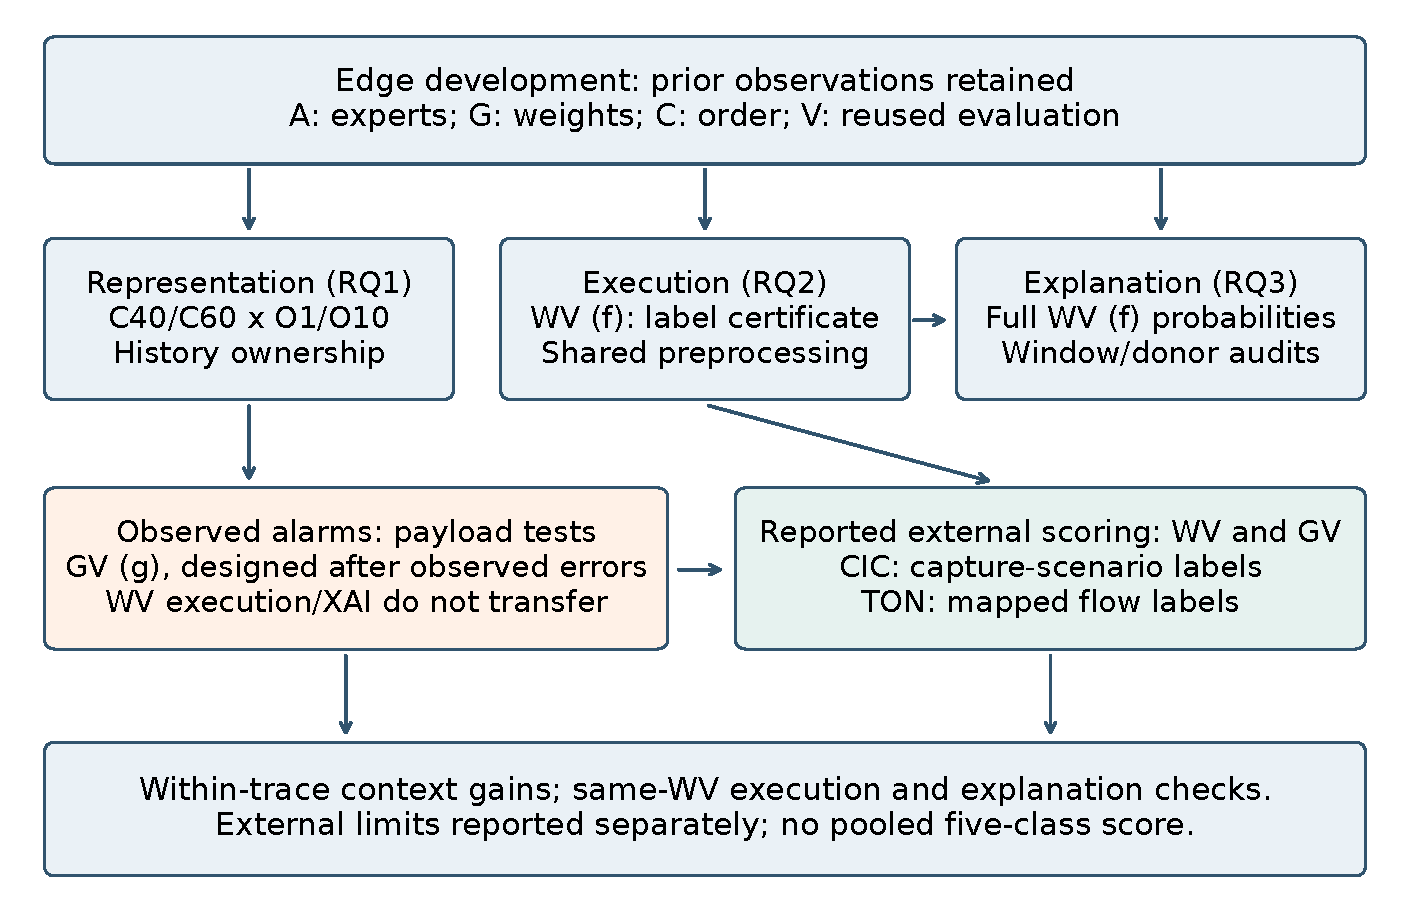
\includegraphics[width=\linewidth]{figures/revision_flow.pdf}\caption{Evaluation flow separating representation (RQ1), execution (RQ2), and explanation (RQ3) from benign false-alarm diagnostics and frozen external scoring. Predictive controls reuse the development targets; function preservation is evaluated separately. Only complete WV probabilities are used for explanation analysis.}\label{fig:main1}\end{figure}

\section{Methods}

\subsection{Bounded multiscale endpoint context}

Endpoint context is constructed from a bounded, prior-only packet history. The state consists of a fixed array of 16,384 records, each containing eight int64 fields, for a 1 MiB record capacity. The logical clock is updated monotonically as \(\max(t_{\rm curr},t_{\rm prev})\), and every target queries the existing buffer before its own record is inserted. This query-before-insertion rule excludes the target packet from its own history summary. The bound concerns the record array rather than the memory needed for model parameters, temporary features, or process execution.

Each retained history is summarized independently for the two endpoints over nested 0.1, 1, and 10 s windows. Within each window, ten statistics describe packet count, total bytes, distinct peers, local and peer TCP-port cardinality (each with log1p transformation), mean and population standard deviation of wire length, and fractions of SYN, ACK, and RST flags. Empty windows or unavailable endpoints produce zero vectors; missing endpoints are not combined into a synthetic host. This yields 30 history statistics per endpoint when all three windows are emitted. Because the summaries use cardinalities rather than raw endpoint identifiers, their interpretation remains focused on recent communication structure.

The representation experiment distinguishes the number of emitted history features from the rule used to assign endpoint slots. With both endpoints and all three windows, C60 emits 60 history fields, which combine with 25 packet fields to form 85 domain fields; C40 emits 40 history fields from 0.1 and 1 s, resulting in 65 domain fields. Two endpoint slots are sorted lexicographically using either the 1 s (O1) or 10 s (O10) window, with a deterministic full-vector rule for ties. The matched 2\(\times\)2 design crosses C40/C60 with O1/O10 and holds targets, model budgets, seeds, resampling, and stage weights fixed within each contrast. As a result, C40/O10 still draws on 10 s history for ordering, although it does not expose the 10 s statistics as explicit prediction fields. The C40-to-C60 comparison therefore estimates the added value of emitted 10 s features conditional on the selected ordering policy; endpoint-swap and consistent valid-port-relabelling invariance claims for C60 hold only with fixed retained buffer membership.

\subsection{Training, reference predictor, and comparative baselines}

Expert training starts from 25 packet attributes, comprising ten numeric and fifteen categorical fields without raw destination ports or explicit port bands. Preprocessing is fitted on A only and uses median imputation, missing-token handling, one-hot encoding with unknown-category tolerance, and a non-centered scaled view for Logistic Regression (LR). In the C60 setting, the 85 domain fields expand to 112 encoded columns. Training then applies random undersampling followed by encoded-space SMOTE \cite{r17}, with synthetic additions capped at 50\% of each pre-RUS class count. The resulting training material contains 30,060 rows, including 4,041 synthetic rows (13.443\%), while G, C, and V remain untouched (Supplementary section \ref*{sup:protocol}).

The fixed ensemble combines five heterogeneous predictors: Decision Tree (DT; maximum depth 12), Random Forest (RF; 75 trees, depth 10) \cite{r18}, XGBoost (100 trees, depth 5) \cite{r19}, LightGBM (150 trees, depth 8) \cite{r16}, and LR (\(C=1\), tolerance \(10^{-6}\), maximum 10,000 iterations). These experts share aligned class labels but retain their fitted parameters and model-specific preprocessing semantics. Their diversity makes WV a useful target for evaluating duplicated encoding, partial expert execution, and complete-probability explanations.

For class c and target x, the reference WV probability and canonical class decision are
\begin{equation} f_c(x)=\sum_{j=1}^{5} w_jp_{jc}(x),\qquad \widehat y_f(x)=\arg\max_c f_c(x).\label{eq:vote}\end{equation}
Weights are constrained to be nonnegative and normalized, ensuring that each component contributes a bounded probability vector. On G, weights are chosen using a heuristic combining macro-F1, a latency/serialized-size proxy, shrinkage toward uniform weights, and a 0.05 minimum weight; a quality coefficient is selected from \{0.5, 0.6, 0.7\} using the mean of macro-F1 and DDoS F2. For seed 42, the reported rounded DT, RF, XGBoost, LightGBM, and LR weights are 0.223950, 0.186478, 0.184082, 0.183980, and 0.221511. Once selected for a stage, these weights define the fixed function used by the serving and explanation experiments.

Comparator experiments characterize the frozen WV predictor without assuming its superiority over individual models. Table 3 reports Gaussian Naive Bayes (GNB) \cite{r26} with default variance smoothing of \(10^{-9}\) and smoothing selected on G from 13 log-spaced candidates (91 fits across seven stages), followed by evaluation on V. Supplementary Table \ref*{sup:comparators} reports per-class recall for WV and GNB. Other historical model comparisons remain in reproducibility artifact R1. Because GNB was introduced after earlier comparator outcomes had been observed, these comparisons are interpreted descriptively rather than as an independent classifier ranking.

\subsection{Prediction-preserving execution contract}

The serving contract exploits a bound on the contribution of experts that have not yet been evaluated. Let E denote the evaluated experts, s\_c their accumulated weighted probability for class c, a the currently leading class, and R the sum of all remaining weights. Every unevaluated component posterior is between zero and one, and every mixture weight is nonnegative. Under these assumptions, the following strict inequality is sufficient to certify that no remaining expert can change the leading class:

\begin{equation}\min_{b\ne a}(s_a-s_b)>R+\tau+\eta,\qquad R=\sum_{j\notin E} w_j.\label{eq:certificate}\end{equation}

For any competing class b, the contribution of unevaluated experts can reduce the partial margin \(s_a-s_b\) by no more than R. Therefore, if the smallest partial margin exceeds R, every possible completion of the remaining probability vectors preserves a as the winner. The implemented condition adds \(\tau =\) \(10^{-12}\) and \(\eta=64\epsilon_{64}\max(1,M)\max(1,\sum_jw_j)\approx7.11\times10^{-14}\), with M = 5 and \(\epsilon_{64}\) = \(2^{-52}\), as numerical safeguards rather than confidence thresholds. Candidate expert orders comprise all 120 permutations and are evaluated on C using retained probabilities and measured costs. The selected order, DT \(\rightarrow\) XGBoost \(\rightarrow\) LightGBM \(\rightarrow\) LR \(\rightarrow\) RF, is then frozen for subsequent serving measurements.

The compact path also removes duplicated feature transformation without modifying any expert. Fitted imputation and sparse CSR one-hot encoding are shared across the five models, while LR receives a derived scaled view with preserved missing-entry and explicit-zero semantics. This optimization is distinct from certified stopping: it accelerates both full-probability and label-only requests, whereas stopping applies only when the caller needs a class decision. The following four operational rules define the contract.

1. Contract validation. Before serving, verify the frozen feature schema, class alignment, nonnegative normalized weights, and sparse/missing-category interpretation.

2. Complete-probability evaluation. When the caller requests probabilities, including for scoring or SHAP coalition values, encode once, evaluate all five experts, and accumulate outputs in canonical order.

3. Selective label evaluation. For label-only requests, traverse experts in the frozen order, update partial class scores and R, and process only rows that remain unresolved.

4. Certified stopping and fallback. Stop a row only after the strict condition in Eq. 2 passes; otherwise evaluate the remaining experts and use the canonical full-sum tie rule. Never expose a certified partial mixture as a complete posterior.

Preservation is checked at both the decision and probability levels because the paths serve different uses. Across 52,684 examined development inputs, compact certified execution produces the same class labels as native WV. This implementation audit is distinct from the 52,584 temporal targets eligible for predictive scoring after the boundary purge. When complete probabilities are requested, native and compact outputs differ by no more than the reported numerical tolerance of \(10^{-12}\). This observation verifies behavior on the tested inputs while the stopping bound supplies the mathematical reason why a certified label cannot be overtaken under the stated assumptions. Neither result should be interpreted as a claim of bitwise-identical posteriors for every conceivable unseen input.

\subsection{Finite-game explanation audits and runtime protocol}

Explanation analysis uses the complete WV posterior rather than the partial scores from certified label-only inference. The main audit selects 100 V targets, balanced at 20 per class, and draws two disjoint sets of 32 background donors from A (A32 and B32). Its nine groups consist of six packet-protocol families (HTTP, TCP, UDP, MQTT, DNS, and ARP) and three history windows, each containing 20 fields. For target x, original predicted class c, donor set B, and coalition S, the game value is
\begin{equation} v^B_{x,c}(S)=\frac{1}{|B|}\sum_{b\in B}f_c(x_S,b_{\bar S}).\label{eq:game}\end{equation}
Omitted groups are replaced jointly from one donor. Exhaustively enumerating the \(2^9=512\) coalitions produces exact Shapley values for the specified finite donor game, checked against additivity, weighted linearity, and SHAP ExactExplainer outputs.

Implementation agreement and explanation robustness are evaluated with different tests. The archived native-versus-compact execution check uses a seven-group, 300-game donor design containing 38,400 coalition values and 1,228,800 donor hybrids. That audit isolates whether two implementations of the same predictor produce the same observed coalition outputs and Shapley values. The principal nine-group A32/B32 study instead examines sensitivity to donor choice through top-three absolute-attribution Jaccard, normalized L1 distance, ordered ranks, and Kendall \(\tau_b\). Changing the grouping changes the underlying cooperative game, so seven-group agreement does not certify every nine-group hybrid.

Intervention faithfulness is measured independently of implementation equality. Rankings computed with A32 define the order in which semantic groups are removed or inserted, whereas the disjoint B32 background supplies the intervention replacements. 
\begin{equation}\Delta_D=A_D^{\mathrm{random}}-A_D^{\mathrm{rank}},\qquad\Delta_I=A_I^{\mathrm{rank}}-A_I^{\mathrm{random}}.\label{eq:gains}\end{equation}
Random-order expectations are computed exactly for the specified procedure. Positive gains therefore indicate that the ranking changes the model probability in the intended direction relative to random ordering. They do not establish causal feature effects or determine whether the original predicted label was correct.

Runtime comparisons use a single Windows laptop (Intel64 Family 6 Model 183, 32 logical CPUs, 16,103.9 MiB RAM) running Python 3.11.15, scikit-learn 1.7.2, XGBoost 3.0.5, LightGBM 4.6.0, and SHAP 0.48.0. Numerical libraries operate in single-threaded mode, and feature timings follow five warm-up calls. Two sessions are retained separately: Session A (3 November 2026), a randomized 30-pair replay comparison of native and compact certified WV, and Session B (17 November 2026), a pre-specified eight-policy serving session. Table 4 reports the four WV native/compact and full/certified policies; artifact R2 retains the complete session. Each replay uses 15,665 packets and 160 decisions, and the latter session includes 30 repetitions per workload. Five cold processes contribute post-load delta peak RSS readings sampled every 2 ms, while paired uncertainty intervals use 10,000 bootstrap resamples (Supplementary section \ref*{sup:serving}). These workstation measurements characterize the implemented software pipeline rather than embedded-device throughput.

\subsection{False-alarm and external transfer diagnostics}

The diagnostic branch first tests whether the reference WV function raises false alarms on benign traffic beyond its main development roles. Nine existing Edge-IIoTset Normal sources contribute samples from the first 100,000 packets at indices 999, 1999, ..., 99999. After warm-up, 867 candidate targets remain; 760 are matched and scorable across eight sources, whereas 107 unmatched targets, including the Modbus candidates, are left unlabelled. We then evaluate decimal alignment of three hexadecimal flag fields and three payload representations: 12 syntax indicators, character 2--5-gram TF-IDF, and their combination within a 4,096-byte limit. These tests diagnose feature-format and payload-information explanations for the observed SQL false alarms.

A function-changing guarded-voting rule is investigated separately after those diagnostics. The GV predictor g substitutes the existing RF posterior when WV predicts SQL and RF predicts Normal, or when WV predicts Normal and RF predicts an attack; otherwise it returns the reference WV posterior f. Rule construction uses the initial benign cohort, later blocks 1--2, and seven already observed attack cohorts (Supplementary section \ref*{sup:diagnostics}). The rule is frozen before scoring later block 3, which contains 697 matched targets from source families encountered previously. Thus, block 3 tests a post-freeze rule on distinct target IDs, not independent source-level transportability.

The external results reported here use the frozen WV and GV functions without fitting new parameters or tuning thresholds. Seven external PCAP files comprise five CICIoT2023 scenarios with 1,000 targets each and two TON\_IoT files contributing 1,000 flow-mapped Normal and 1,000 flow-mapped Ransomware targets each, for 9,000 unique rows and 18,000 reported WV/GV decisions. These outputs are a subset of the archived 27,000-decision session; the additional component diagnostic is retained in artifact R4. Features are reconstructed from raw PCAPs with TShark 4.4.9 using the 85-field scheme and resetting context at each file boundary. CICIoT2023 labels refer to assigned capture scenarios, whereas TON\_IoT labels are uniquely associated with author-labelled bidirectional flows within \([t_s,t_s+d+1\,\mathrm{s})\). Consequently, results retain the semantics and coverage of their source dataset and are not combined into an undifferentiated five-class score (Supplementary section \ref*{sup:diagnostics}).

\section{Results}

\subsection{Context scale gains and history dependence (RQ1)}

The matched factorial in Table 1 and Figure 2 shows that explicitly emitting 10 s history statistics improves within-trace temporal macro-F1 under either endpoint-ordering policy. Under O1, the three-seed mean rises from 96.7363\% with C40 to 97.8787\% with C60; under O10, it rises from 96.7479\% to 97.8954\%. These paired contrasts correspond to approximately 1.14--1.15 percentage points, whereas switching O1 to O10 at a fixed feature scale changes macro-F1 by less than 0.02 points. Under O1, the mean number of Port Scanning errors declines from 83 to 61 and Ransomware errors from 147 to 82. The comparison isolates emitted 10 s features conditional on ordering, because C40/O10 itself still uses a 10 s slot-ordering key.

The signature-disjoint diagnostic shows a larger difference between emitted time scales but requires a narrower interpretation. C40 achieves about 71.84\% pooled macro-F1, whereas the two C60 configurations exceed 97.29\%. Within C60, O1 gives 97.4512\%, slightly above the O10 value of 97.2955\%, so the longer ordering key is not uniformly better. Since exact target signatures are separated but the preceding unlabeled stream may remain shared, these figures measure robustness to a constrained signature split rather than independent capture environments. The C60/O10 configuration is carried forward as the frozen RQ2--RQ3 reference; it is not reselected on this diagnostic.

\begin{table}[H]\centering\small\setlength{\tabcolsep}{3pt}\renewcommand{\arraystretch}{1.13}
\caption{Matched 2\(\times\)2 context/ordering ablation with fixed per-stage reference weights.}\label{tab:factorial}
\begin{tabular}{L{0.18\dimexpr\textwidth-12\tabcolsep\relax}L{0.16\dimexpr\textwidth-12\tabcolsep\relax}L{0.16\dimexpr\textwidth-12\tabcolsep\relax}L{0.14\dimexpr\textwidth-12\tabcolsep\relax}L{0.18\dimexpr\textwidth-12\tabcolsep\relax}L{0.18\dimexpr\textwidth-12\tabcolsep\relax}}\toprule
\textbf{Context / Order} & \textbf{Temporal F1 (\%)} & \textbf{Temporal BA (\%)} & \textbf{Mean Errors} & \textbf{Signature F1 (\%)} & \textbf{Signature Errors}\\\midrule
C40 / O1 & 96.7363 & 96.9240 & 283.00 & 71.8438 & 9,746\\
C40 / O10 & 96.7479 & 96.9398 & 282.00 & 71.8424 & 9,745\\
C60 / O1 & 97.8787 & 97.9820 & 187.00 & 97.4512 & 1,100\\
C60 / O10 & 97.8954 & 98.0030 & 184.67 & 97.2955 & 1,167\\
\bottomrule\end{tabular}
\end{table}

Temporal: three-seed means on the same 10,358 V targets (macro-F1 SDs: 0.0342, 0.0378, 0.0077, 0.0145 percentage points). Signature: pooled two-fold diagnostic on 52,584 targets. C40 emits 0.1/1 s history statistics; C60 additionally emits 10 s statistics. O1/O10 select 1/10 s endpoint slot-ordering keys, respectively. C40/O10 is not independent of 10 s information because ordering uses the 10 s key. Per-seed recalls are retained in artifact R1 (Supplementary section \ref*{sup:protocol}).

\begin{figure}[H]\centering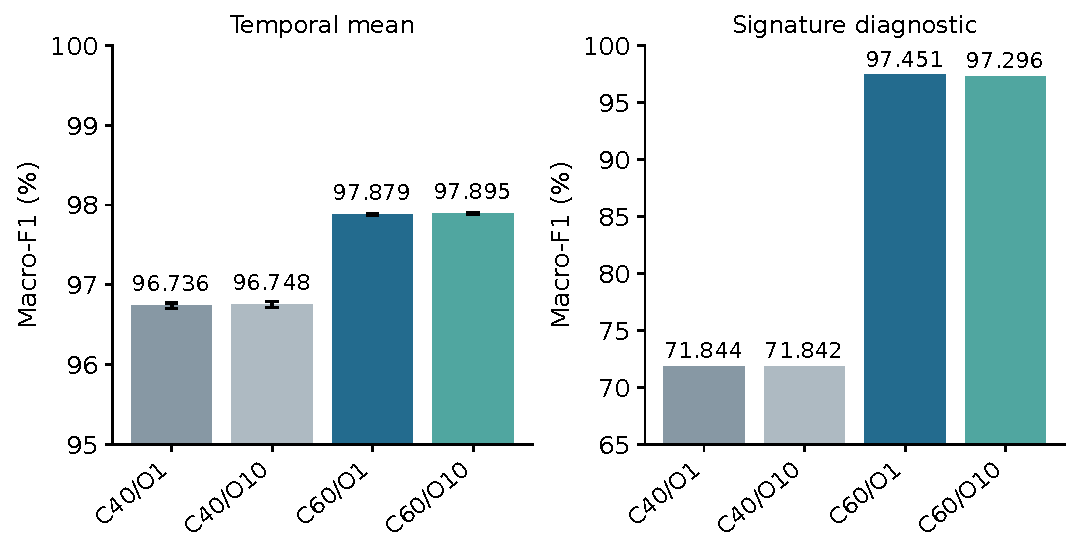
\includegraphics[width=\linewidth]{figures/revision_factorial.pdf}\caption{Matched C40/C60 \(\times\) O1/O10 ablation showing temporal macro-F1 across three fitting seeds (left, sample-SD error bars) and pooled two-fold signature-disjoint results (right). C40/O10 uses 10 s history for slot ordering, but does not emit 10 s context features.}\label{fig:main2}\end{figure}

The ownership experiments in Table 2 test whether the signature result depends on the traffic available to history construction. Replacing full shared history with packet-private history reduces macro-F1 from 97.2955\% to 93.7694\% and lowers Scanning and Ransomware recall to 83.7328\% and 81.2851\%, respectively. Matched shared-density history yields an even lower macro-F1 of 93.5804\%, showing that density reduction and warm-up behavior affect the result in addition to which packets share context. The comparison therefore establishes context-allocation sensitivity but does not quantify label leakage as a single identified mechanism.

Ring capacity provides a separate check on the bounded-memory design. Over 0.25, 1, and 4 MiB settings, temporal WV predictions remain identical and signature macro-F1 ranges only from 97.2903\% to 97.2973\%. The 1 MiB DDoS buffer nevertheless records 1,954,616 capacity evictions, indicating that a nominal 10 s window may contain less than ten seconds of high-rate history. Across the tested capacities, the reported predictions and signature scores remain stable despite the observed eviction pressure (Supplementary section \ref*{sup:protocol}).

\begin{table}[H]\centering\small\setlength{\tabcolsep}{3pt}\renewcommand{\arraystretch}{1.13}
\caption{Signature-split history-ownership controls under unchanged modeling budget and reference weights.}\label{tab:history}
\begin{tabular}{L{0.21\dimexpr\textwidth-12\tabcolsep\relax}L{0.15\dimexpr\textwidth-12\tabcolsep\relax}L{0.16\dimexpr\textwidth-12\tabcolsep\relax}L{0.14\dimexpr\textwidth-12\tabcolsep\relax}L{0.18\dimexpr\textwidth-12\tabcolsep\relax}L{0.16\dimexpr\textwidth-12\tabcolsep\relax}}\toprule
\textbf{History} & \textbf{Macro-F1 (\%)} & \textbf{Bal. acc. (\%)} & \textbf{Scan recall (\%)} & \textbf{Ransom. recall (\%)} & \textbf{Errors}\\\midrule
Full shared & 97.2955 & 97.3609 & 94.8342 & 92.7042 & 1,167\\
Shared-density & 93.5804 & 92.5888 & 83.1616 & 80.6322 & 3,174\\
Packet-private & 93.7694 & 92.8322 & 83.7328 & 81.2851 & 3,071\\
\bottomrule\end{tabular}
\end{table}

Evaluated on the same 52,584 signature-diagnostic targets; experts are refitted without retuning. Shared-density and packet-private controls match marginal allocation probabilities (Supplementary section \ref*{sup:protocol}; artifact R1).

\subsection{Predictive comparators and function-preserving serving (RQ2)}

Before evaluating execution efficiency, Table 3 characterizes the predictive behavior of the fixed WV reference through the GNB comparison. On the temporal evaluation, default GNB reaches 82.61\% macro-F1 and G-selected GNB reaches 95.05\%, compared with 97.90\% for WV. GNB smoothing also reduces its Normal false-positive rate from 48.60\% to 7.05\%, although WV remains at 0.92\% on the reported comparison. Under private-history and shared-signature diagnostics, selected GNB falls to 43.92\% and 49.53\% macro-F1 with zero DDoS recall. These results indicate strong sensitivity of the GNB comparator to correlated context and encoded inputs, rather than establishing an inherent advantage of ensembles.

Artifact R1 contains broader historical classifier comparisons, including runs with higher predictive scores than WV on packet-private and temporal evaluations. The present serving experiment holds WV fixed so that the measurements in Table 4 isolate implementation preservation and computational cost.

\begin{table}[H]\centering\small\setlength{\tabcolsep}{3pt}\renewcommand{\arraystretch}{1.13}
\caption{Reference WV and GNB comparators across temporal and signature-based evaluation regimes.}\label{tab:ensemble}
\begin{tabular}{L{0.17\dimexpr\textwidth-14\tabcolsep\relax}L{0.22\dimexpr\textwidth-14\tabcolsep\relax}L{0.11\dimexpr\textwidth-14\tabcolsep\relax}L{0.11\dimexpr\textwidth-14\tabcolsep\relax}L{0.15\dimexpr\textwidth-14\tabcolsep\relax}L{0.12\dimexpr\textwidth-14\tabcolsep\relax}L{0.12\dimexpr\textwidth-14\tabcolsep\relax}}\toprule
\textbf{Evaluation} & \textbf{Predictor} & \textbf{F1 (\%)} & \textbf{BA (\%)} & \textbf{Normal FPR (\%)} & \textbf{DDoS F2 (\%)} & \textbf{Errors}\\\midrule
Temporal & WV (reference) & 97.90 & 98.00 & 0.92 & 100.00 & 184.67\\
Temporal & GNB (default) & 82.61 & 86.25 & 48.60 & 99.95 & 2,207.00\\
Temporal & GNB (G-selected) & 95.05 & 95.88 & 7.05 & 99.95 & 506.00\\
Private history & WV (reference) & 93.77 & 92.83 & 0.50 & 100.00 & 3,071\\
Private history & GNB (default) & 43.88 & 46.53 & 19.16 & 0.00 & 24,113\\
Private history & GNB (G-selected) & 43.92 & 46.74 & 17.69 & 0.00 & 23,864\\
Shared signature & WV (reference) & 97.30 & 97.36 & 0.48 & 99.98 & 1,167\\
Shared signature & GNB (default) & 39.83 & 41.15 & 19.94 & 0.00 & 26,546\\
Shared signature & GNB (G-selected) & 49.53 & 51.13 & 22.40 & 0.00 & 22,653\\
\bottomrule\end{tabular}
\end{table}

Temporal results are three-seed means on 10,358 V targets (macro-F1 SDs for WV, default GNB, and selected GNB: 0.0145, 0.0043, and 0.0485 percentage points). Signature results pool two folds on 52,584 targets. Supplementary Table \ref*{sup:comparators} gives per-class recall for these predictors; broader historical comparisons are retained in artifact R1.

With the predictive context of the reference function established, the serving audit examines implementation preservation. Across the 52,684 development inputs, compact certified WV reproduces every native class decision while evaluating a mean of 3.0715 of five experts per label-only decision. When a complete probability vector is requested, native and compact paths agree within \(10^{-12}\) on the measured inputs. These results align with the formal stopping condition: early exit reduces evaluation work only where a remaining-weight certificate secures the class winner. Table 4 then quantifies the practical benefit under Session B (17 November 2026).

In the 30-repeat replay workload, native full serving averages 2.8265 s and compact certified serving averages 1.1150 s, a 60.55\% reduction. Relative to native certified serving at 1.7811 s, compact certified serving saves 37.40\% or 0.6661 s per replay (95\% paired-bootstrap CI [0.6234, 0.7146] s).

Compact full serving averages 1.5578 s, demonstrating that encoding reuse improves even the path where all expert probabilities remain necessary. The crossed design produces an estimated encoding-by-stopping interaction of about 0.60 s (95\% CI [0.5347, 0.6733] s; Supplementary section \ref*{sup:serving}), so component savings should not be treated as additive. These timings describe model-serving paths, not end-to-end generation of complete SHAP explanations.

\begin{table}[H]\centering\small\setlength{\tabcolsep}{3pt}\renewcommand{\arraystretch}{1.13}
\caption{WV serving ablation in Session B (17 November 2026), the controlled eight-policy session.}\label{tab:runtime}
\begin{tabular}{L{0.24\dimexpr\textwidth-12\tabcolsep\relax}L{0.14\dimexpr\textwidth-12\tabcolsep\relax}L{0.15\dimexpr\textwidth-12\tabcolsep\relax}L{0.16\dimexpr\textwidth-12\tabcolsep\relax}L{0.14\dimexpr\textwidth-12\tabcolsep\relax}L{0.17\dimexpr\textwidth-12\tabcolsep\relax}}\toprule
\textbf{WV Serving Policy} & \textbf{1-Row (ms)} & \textbf{1,000-Row (ms)} & \textbf{Feature Delta (MiB)} & \textbf{Replay (s)} & \textbf{Replay Delta (MiB)}\\\midrule
WV native / full & 17.480 & 61.089 & 2.147 & 2.8265 & 4.748\\
WV native / certified & 8.738 & 56.615 & 2.758 & 1.7811 & 4.171\\
WV compact / full & 7.946 & 48.669 & 2.362 & 1.5578 & 4.338\\
WV compact / certified & 5.219 & 43.515 & 2.520 & 1.1150 & 3.909\\
\bottomrule\end{tabular}
\end{table}

Feature latency: median of 30 calls after 5 warm-ups; feature delta RSS refers to 1,000-row batch. Replay: mean of 30 repetitions over 15,665 packets / 160 decisions. RSS: mean post-load delta peak across 5 cold processes sampled every 2 ms. Supplementary Table \ref*{sup:serving} gives matched WV replay contrasts; artifact R2 retains the complete serving controls.

The earlier Session A (3 November 2026) provides a separate check on the direction of the serving gain. In its randomized 30-pair comparison, mean replay time decreases from 1.5791 s for native certified WV to 0.9198 s for compact certified WV, a 41.75\% reduction (Figure 3; Supplementary section \ref*{sup:serving}). The paired mean saving is 0.6593 s, with a 95\% interval of [0.5965, 0.7313] s; medians are 1.5135 and 0.9310 s, with corresponding standard deviations of 0.2243 and 0.1137 s. All 30 paired differences favor compact execution. An earlier five-pair archive nevertheless contains one slower compact repetition, for which the retained operating-system telemetry does not establish a cause. These sessions are reported separately because they differ in measurement scope; the later evidence does not retrospectively explain the earlier reversal. Previously evaluated optimized single-model paths remain faster on prepared batches (artifact R2), which does not change the preservation result for fixed WV.

\begin{figure}[H]\centering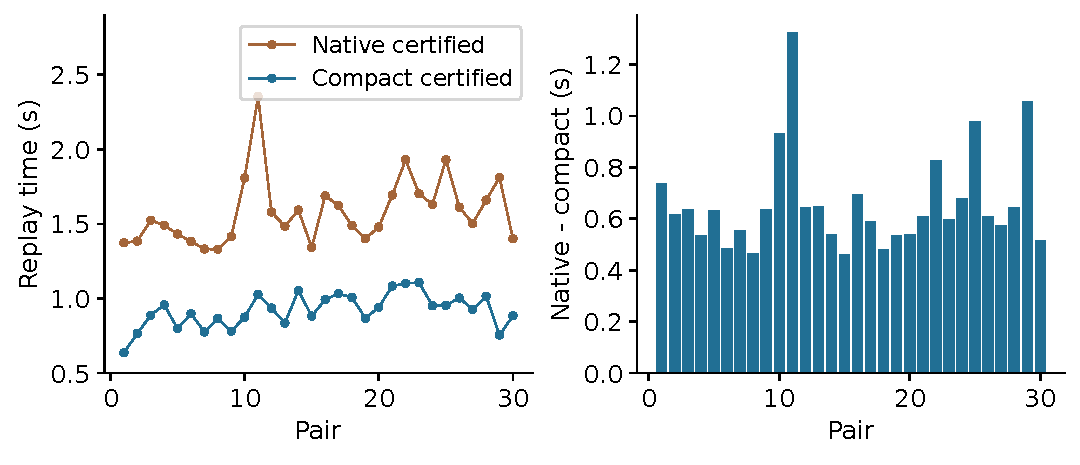
\includegraphics[width=\linewidth]{figures/revision_runtime.pdf}\caption{Thirty paired replay measurements from Session A (3 November 2026), with randomized native-versus-compact execution order within each pair. The left panel shows paired replay times for native certified and compact certified WV; the right panel gives their paired differences. Positive differences indicate faster compact execution on the measured workload.}\label{fig:main3}\end{figure}

\subsection{Explanation consistency, sensitivity, and faithfulness (RQ3)}

The archived seven-group test addresses implementation consistency directly. Across 300 games, comprising 38,400 coalition values and 1,228,800 donor hybrids, native and compact full-posterior execution produce identical observed coalition outputs and derived Shapley attributions. The comparison also satisfies additivity and weighted-linearity checks. It therefore supports equivalence of those tested finite games, without certifying all possible inputs or the separate nine-group game. This distinction establishes the first component of RQ3 before evaluating explanation behavior under different donors.

The nine-group experiment examines the distribution of attributed importance across feature families. Using the A32 donors and 100 V targets, the 10 s history window contributes 84.49\% of mean absolute attribution share, compared with 8.86\% for 1 s, 5.21\% for 0.1 s, and 1.44\% in total across the six protocol families (Figure 4). Under the specified B32 interventions, the resulting ranking yields deletion and insertion gains of 0.3203 and 0.3270 (Table 5). The values indicate that the grouped ranking changes the model's predicted-class probability more than random order under these interventions. They do not directly validate attack labels or establish a causal contribution of the history windows.

\begin{table}[H]\centering\small\setlength{\tabcolsep}{3pt}\renewcommand{\arraystretch}{1.13}
\caption{Nine-group cross-background explanation faithfulness audit (100 V targets).}\label{tab:faith}
\begin{tabular}{L{0.25\dimexpr\textwidth-10\tabcolsep\relax}L{0.18\dimexpr\textwidth-10\tabcolsep\relax}L{0.18\dimexpr\textwidth-10\tabcolsep\relax}L{0.195\dimexpr\textwidth-10\tabcolsep\relax}L{0.195\dimexpr\textwidth-10\tabcolsep\relax}}\toprule
\textbf{Predictor} & \textbf{Deletion AUC} & \textbf{Insertion AUC} & \textbf{Deletion gain} & \textbf{Insertion gain}\\\midrule
Weighted voting (WV) & 0.2600 & 0.9073 & 0.3203 & 0.3270\\
\bottomrule\end{tabular}
\end{table}

Signed rankings computed on A32 donor background; interventions executed on disjoint B32 background. Gains represent probability-area improvements over exact random-order expectation. Supplementary Table \ref*{sup:explanation} records the WV audit; historical explanation controls remain in artifact R3. No superiority over other predictors is inferred.

\begin{figure}[H]\centering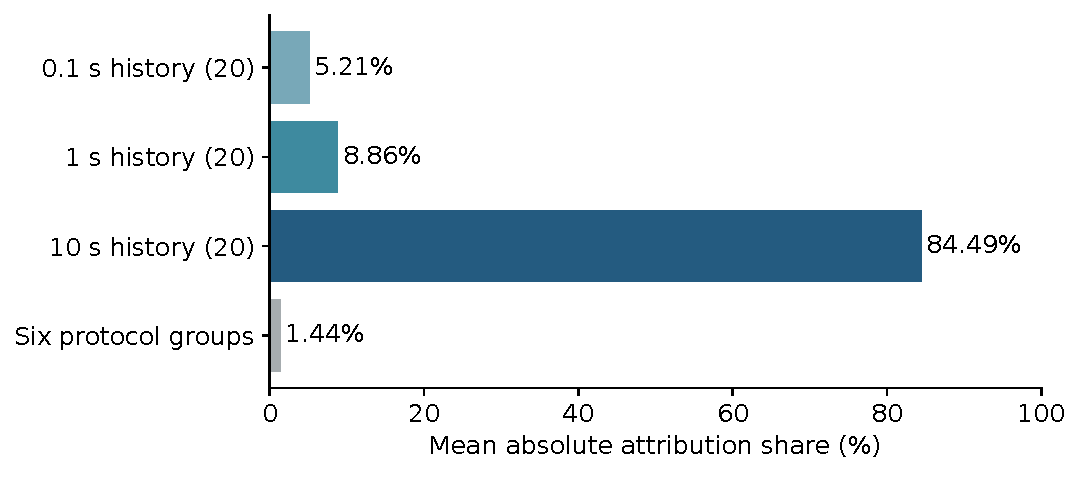
\includegraphics[width=\linewidth]{figures/revision_xai.pdf}\caption{Mean absolute attribution shares for the nine-group A32 donor game across 100 V targets. Each history window contains 20 fields; the six packet-protocol groups are combined for display.}\label{fig:main4}\end{figure}

Background replacement changes attribution magnitudes and some rankings even when the leading groups are stable. Across the A32/B32 nine-group comparison, top-three membership is identical (Jaccard 1.0000) and the top-ranked group is unchanged for all 100 targets. Nevertheless, normalized L1 distance is 0.028066, a top-three order swap is observed, and mean full-rank Kendall \(\tau_b\) is 0.8320, with a minimum of 0.6789 (Supplementary section \ref*{sup:explanation}). Under the archived seven-group definition, top-three Jaccard is 0.5520 despite cosine similarity of 0.999948. This difference is not a contradiction between repeat measurements: changing group boundaries defines a different cooperative game and a different object of attribution.

Correctness-stratified results reinforce the distinction between explanatory fidelity and predictive correctness. Among 97 correctly classified targets, deletion and insertion gains are 0.3250 and 0.3296; among the three misclassified targets, the observed gains are 0.1692 and 0.2430 (Supplementary section \ref*{sup:explanation}). These positive values show that an attribution can track the predictor's behavior even when the predictor is wrong about the label. However, three errors are insufficient to characterize general faithfulness behavior on misclassified traffic. Accordingly, RQ3 supports finite-game implementation and intervention findings under the stated donor choices, rather than a general explanation guarantee.

\subsection{Stress-testing: false alarms, local repair, and external boundaries}

Beyond the three engineering audits, the benign stress test reveals a substantial predictive error mode that the main temporal score does not expose. On 760 matched Normal targets from additional existing Edge-IIoTset sources, WV raises 324 SQL false alarms (42.63\%), concentrated in five sensor sources, while its retained RF component raises none (Supplementary section \ref*{sup:diagnostics}). Converting three hexadecimal flag fields to decimal reduces WV false alarms only to 321/760 (42.24\%). Among these aligned errors, the combined weighted SQL-minus-Normal contributions from DT, LR, and LightGBM exceed the offsetting RF and XGBoost contribution by a mean margin of +0.0998. This decomposition locates the disagreement in the existing ensemble rather than attributing all errors to flag encoding.

Adding payload features does not resolve the observed benign failure. Of the 321 aligned false alarms, 257 correspond to packets without TCP payload. Refits using syntax indicators, character n-gram TF-IDF, and the combined representation still produce 310, 312, and 331 false alarms, respectively. Those changes also increase V attack-to-Normal misses from two to three or four (Supplementary section \ref*{sup:diagnostics}). The mixed result motivates a separate rule-based diagnostic, but it does not justify changing the verified WV function without explicitly re-evaluating that new predictor.

Guarded voting is therefore reported as a local repair experiment rather than as a continuation of RQ2. After the rule is specified using the initial benign cohort and blocks 1--2, it reduces post-freeze block 3 false alarms from 396/697 for WV (56.8149\%) to 1/697 for GV (0.1435\%), matching RF on scored targets (Table 6). Counting all three unmatched candidates as alarms gives a conservative coverage bound of 4/700 (0.5714\%). However, the block uses new target IDs from source families already represented in rule development. On reused V Normal observations, GV increases false-positive rate from 36/3,860 (0.9326\%) to 39/3,860 (1.0104\%) and reduces macro-F1 from 97.8800\% to 97.8503\%. Two previously Scan-to-Normal errors instead become Scan-to-Ransomware predictions, leaving typed attack recalls unchanged. The results support source-conditioned alarm mitigation rather than independent new-source generalization.

\begin{table}[H]\centering\small\setlength{\tabcolsep}{3pt}\renewcommand{\arraystretch}{1.13}
\caption{Benign false-alarm diagnostics comparing reference WV and guarded GV across evaluation roles.}\label{tab:guard_fpr}
\begin{tabular}{L{0.2\dimexpr\textwidth-10\tabcolsep\relax}L{0.08\dimexpr\textwidth-10\tabcolsep\relax}L{0.22\dimexpr\textwidth-10\tabcolsep\relax}L{0.22\dimexpr\textwidth-10\tabcolsep\relax}L{0.28\dimexpr\textwidth-10\tabcolsep\relax}}\toprule
\textbf{Cohort} & \textbf{n} & \textbf{WV: FP (FPR)} & \textbf{GV: FP (FPR)} & \textbf{Evaluation Role}\\\midrule
Initial benign & 760 & 321 (42.2368\%) & 0 (0.0000\%) & Observed before rule\\
Later block 1 & 769 & 401 (52.1456\%) & 0 (0.0000\%) & Observed before rule\\
Later block 2 & 699 & 407 (58.2260\%) & 0 (0.0000\%) & Observed before rule\\
Later block 3 & 697 & 396 (56.8149\%) & 1 (0.1435\%) & Frozen before scoring\\
V Normal & 3,860 & 36 (0.9326\%) & 39 (1.0104\%) & Reused validation\\
\bottomrule\end{tabular}
\end{table}

FPR is computed over Normal support. The initial benign row reports the post-alignment count (321/760 false alarms); the pre-alignment count was 324/760. The V Normal row uses the frozen seed-42 reference fit, whereas Tables 1 and 3 report three-seed temporal means. Later blocks contain distinct target IDs from previously used Edge-IIoTset sources. RF-component results are retained in artifact R4 (Supplementary section \ref*{sup:diagnostics}).

Frozen external evaluation places the local GV repair in a different traffic setting. On CICIoT2023 Normal targets, GV increases false-positive rate from 30.15\% for WV to 31.90\%; on flow-mapped TON\_IoT Normal targets, it reduces the rate from 24.35\% to 18.85\% (Table 7; Figure 5). The guard removes 27 CIC Normal alarms but introduces 62, whereas on TON it removes 205 and introduces 95. In the CIC Scan and SYN scenario cohorts, Normal predictions rise from 465 and 2 under WV to 555 and 12 under GV, respectively. Because CIC labels denote capture-scenario assignments, these counts are diagnostics rather than confirmed packet-level attack misses. The direction and consequences of expert switching therefore depend on the source environment, and the findings cannot be interpreted as generalizable alarm repair.

Detection of flow-mapped TON\_IoT Ransomware remains particularly weak after the repair. GV assigns the Normal class to 1,657 of 2,000 Ransomware targets (82.85\%), leaving a binary alarm recall of 17.15\% and correct-type recall of only 1.55\%; WV predicts Normal for 1,630 such targets and has 1.35\% correct-type recall. All-packet in-scope mapping coverage is 62.90\% and 6.66\% for the two TON files when warm-up packets remain in the denominator (Supplementary section \ref*{sup:diagnostics}). These coverage and label constraints limit population-level interpretation, but they do not remove the observed weakness of the frozen classifiers on the selected external rows. The external tests therefore restrict deployment claims rather than disproving the separate execution-preservation result.

\begin{table}[H]\centering\small\setlength{\tabcolsep}{3pt}\renewcommand{\arraystretch}{1.13}
\caption{Frozen external stress-test results on CICIoT2023 and TON\_IoT (retaining dataset-specific label scopes).}\label{tab:transfer}
\begin{tabular}{L{0.32\dimexpr\textwidth-10\tabcolsep\relax}L{0.08\dimexpr\textwidth-10\tabcolsep\relax}L{0.26\dimexpr\textwidth-10\tabcolsep\relax}L{0.17\dimexpr\textwidth-10\tabcolsep\relax}L{0.17\dimexpr\textwidth-10\tabcolsep\relax}}\toprule
\textbf{External Target Cohort} & \textbf{n} & \textbf{Metric} & \textbf{WV (\%)} & \textbf{GV (\%)}\\\midrule
CICIoT2023 Normal & 2,000 & Normal FPR & 30.15 & 31.90\\
TON\_IoT Normal (flow-mapped) & 2,000 & Normal FPR & 24.35 & 18.85\\
CICIoT2023 SQL & 1,000 & Scenario match & 29.80 & 32.10\\
CICIoT2023 Scan & 1,000 & Scenario match & 3.80 & 4.00\\
CICIoT2023 SYN & 1,000 & Scenario match & 62.10 & 62.10\\
TON\_IoT Ransomware (flow-mapped) & 2,000 & Correct-type recall & 1.35 & 1.55\\
\bottomrule\end{tabular}
\end{table}

Zero external fitting or threshold tuning. CIC attack labels denote capture-scenario assignments; TON labels derive from uniquely matched bidirectional flows. Supplementary Table \ref*{sup:diagnostics} summarizes the reported WV/GV results; artifact R4 retains per-file results and the complete component diagnostics.

\begin{figure}[H]\centering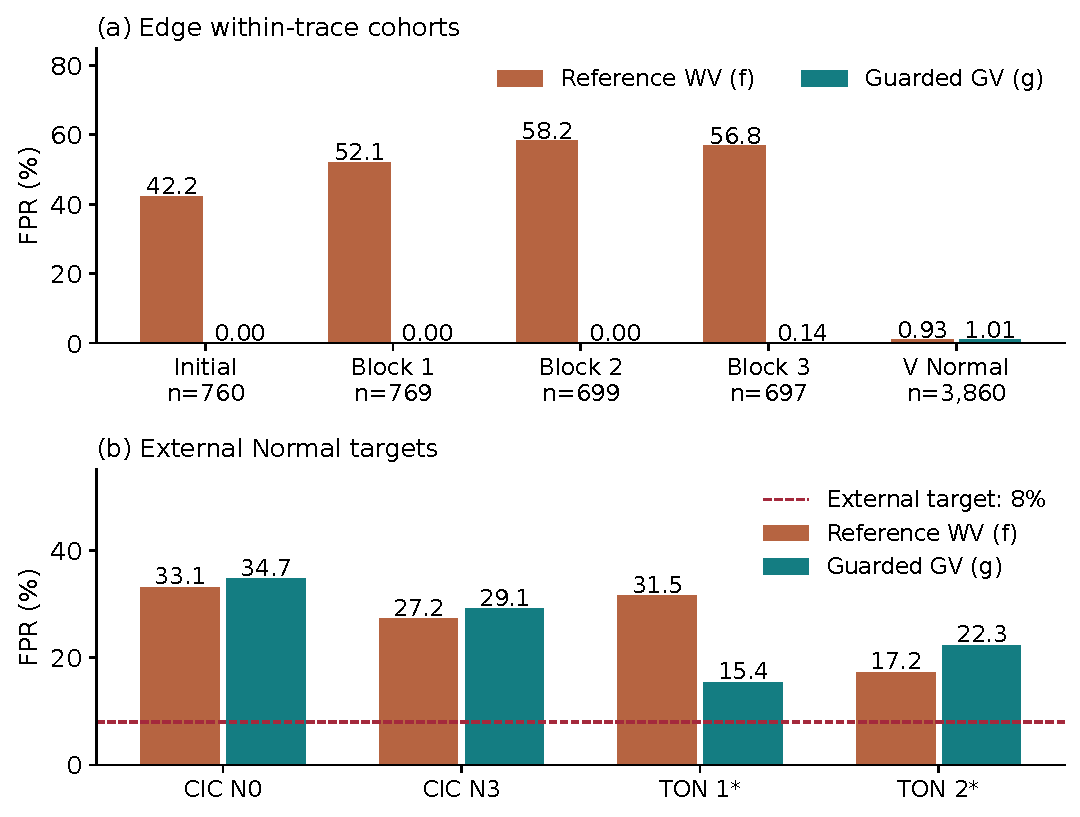
\includegraphics[width=\linewidth]{figures/revision_fpr_transfer.pdf}\caption{Reference WV and guarded-voting Normal false-positive rates across (a) Edge-IIoTset benign cohorts and (b) individual external Normal files: CIC N0, CIC N3, TON 1*, and TON 2*. The initial cohort and blocks 1--2 informed the guard, block 3 was scored after freezing, and V was reused. Asterisks denote uniquely flow-mapped TON targets.}\label{fig:main5}\end{figure}

\section{Discussion}

\subsection{Representation gains versus history sensitivity (RQ1)}

RQ1 identifies a measurable benefit from emitting longer endpoint statistics, but the benefit has a specific evaluation meaning. Across both fixed ordering policies, extending C40 to C60 adds approximately 1.14--1.15 percentage points of temporal macro-F1 without increasing the 1 MiB record-array budget. Because C40/O10 still uses 10 s history to assign endpoint slots, the estimated effect concerns additional emitted features rather than the presence or absence of all long-window information. The packet-private and shared-density diagnostics then show that some apparent signature robustness depends on traffic allocation, density, and history warm-up. These observations strengthen the interpretation of a bounded within-trace feature gain while withholding claims of attack-signature independence or quantified leakage.

\subsection{Practical value of prediction-preserving execution (RQ2)}

RQ2 establishes that serving efficiency and prediction preservation can be evaluated together for the tested WV function. Shared fitted encoding avoids redundant transformations, and the remaining-weight certificate omits expert calls once the winning class is secured. Their combination reduces replay time by 60.55\% relative to native full execution and 37.40\% relative to native certified execution. All tested development labels remain unchanged, and requested full posteriors agree within \(10^{-12}\); the mathematical stopping condition establishes why the certified label is preserved. The 1 MiB memory limit covers the endpoint-history record array, whereas Table 4 separately reports post-load incremental RSS for the serving paths. The 15,665-packet replay with 160 decisions provides a matched basis for comparing those implementations. Complete SHAP generation and embedded-device throughput were not benchmarked. Faster singleton RF/LR controls on prepared batches also indicate that WV should be retained when its mixture behavior is needed.

\subsection{Auditable XAI: separating consistency, sensitivity, and faithfulness (RQ3)}

RQ3 demonstrates why an explanation audit must specify both its software target and its feature-intervention game. The seven-group re-execution verifies that native and compact versions produce the same observed coalition values for the archived test, protecting those explanations from implementation-induced drift in that setting. The separate nine-group study reveals that top-three agreement can conceal changes in secondary ordering and that changing feature groups changes the attribution estimand. Positive deletion/insertion gains characterize intervention-specific faithfulness to the reference probability; the three misclassified observations provide only limited evidence about faithfulness conditioned on incorrect decisions. An auditable IDS consequently requires both explanation consistency checks and independent assessment of predictive behavior under distribution shift.

\subsection{Local repair versus cross-dataset shift}

The GV results illustrate the difference between correcting a local error pattern and obtaining a transportable detector. Its post-freeze reduction to one false alarm among 697 matched benign targets is substantial, but all of those targets come from previously encountered source families. When applied without retuning to CICIoT2023, the same rule increases Normal FPR, whereas on flow-mapped TON\_IoT it decreases benign FPR but still classifies most Ransomware targets as Normal. Protocol composition, endpoint context, and differing scenario-versus-flow labels can change how often RF and WV disagree and whether switching helps. Therefore, the GV branch diagnoses the limits of a source-conditioned repair; it does not inherit WV's execution certificate or establish readiness for new deployment environments.

\section{Conclusion}

This study addresses three connected engineering objectives through matched weighted-voting representations and a subsequently fixed five-expert WV reference for execution and explanation. For RQ1, explicit 10 s endpoint statistics improve within-trace temporal macro-F1 by approximately 1.14--1.15 percentage points under matched ordering policies, while ownership controls reveal dependence on surrounding traffic context. For RQ2, shared preprocessing and certified early termination preserve every tested development label, match requested complete posteriors within \(10^{-12}\), and reduce mean replay time by 60.55\% against native full serving and 37.40\% against native certified serving. For RQ3, the archived seven-group finite-game audit establishes observed native--compact explanation consistency, while a distinct nine-group donor analysis characterizes attribution stability and deletion/insertion gains of 0.3203/0.3270. Together, these results demonstrate how bounded context construction, efficient serving, and explanation verification can be studied under explicitly specified evaluation protocols.

The diagnostic branch identifies an important limit on those achievements. A frozen GV rule reduces benign false alarms to 1/697 within previously observed source families but does not eliminate cross-dataset failures: GV Normal false-positive rates reach 31.90\% on CICIoT2023 and 18.85\% on flow-mapped TON\_IoT, with only 1.55\% correct-type recall for TON Ransomware. These observations do not negate the exact-function serving result; they show that preserving a function is different from validating that function in a new environment. The principal contribution is a reproducible, bounded verification workflow; cross-domain deployment requires separate validation. Future work should test domain-adaptive predictors and constrained hardware using independently acquired source-level evaluations.

\section*{Data and Software Availability}

Edge-IIoTset is distributed through IEEE DataPort \cite{r1}, CICIoT2023 through the University of New Brunswick (UNB) \cite{r27}, and TON\_IoT through the University of New South Wales (UNSW) \cite{r28,r30}. The reproducibility evidence is organized into four groups (R1--R4) in the public repository https://github.com/hafidramadhan22-prog/array-multiscale-iot-evidence (release qc-20261121). The package comprises code, frozen configurations, SHA256 manifests, split and target identifiers, saved model probabilities and labels, explanation arrays, raw replay-time and memory logs, and derived external-label mappings. Its archive index identifies individual files by relative path and checksum; the saved-results entry point verifies selected observations without refitting estimators or deserializing trained models. The supplementary material summarizes the protocols and key evidence in Sections \ref*{sup:protocol}--\ref*{sup:diagnostics} and Tables \ref*{sup:protocol}--\ref*{sup:diagnostics}, with the detailed observations indexed in R1--R4. Full third-party datasets are not redistributed; reproducing raw-PCAP extraction requires access to the provider datasets, the applicable permissions, and the documented processing environment.

\section*{Funding \& Competing Interests}

Funding: This research did not receive any specific grant from funding agencies in the public, commercial, or not-for-profit sectors.

Declaration of competing interests: The authors declare that they have no known competing financial interests or personal relationships that could have appeared to influence the work reported in this paper.

CRediT authorship contribution statement: M Hafid Ramadhan: Software, Investigation, Formal analysis, Visualization, Writing -- original draft. Satria Mandala: Supervision, Methodology, Validation, Writing -- review \& editing.

\section*{Declaration of generative AI and AI-assisted technologies in the manuscript preparation process}

During the preparation of this manuscript, the authors used ChatGPT (OpenAI) to support translation and to improve readability, language clarity, and phrasing consistency in the presentation of results. The authors reviewed and edited the AI-assisted content as needed and take full responsibility for the content of the published article.

\bibliographystyle{elsarticle-num}

\bibliography{references}

\end{document}